% Options for packages loaded elsewhere
\PassOptionsToPackage{unicode}{hyperref}
\PassOptionsToPackage{hyphens}{url}
\PassOptionsToPackage{dvipsnames,svgnames,x11names}{xcolor}
%
\documentclass[
  letterpaper,
  number,
  review,
  3p]{elsarticle}

\usepackage{amsmath,amssymb}
\usepackage{iftex}
\ifPDFTeX
  \usepackage[T1]{fontenc}
  \usepackage[utf8]{inputenc}
  \usepackage{textcomp} % provide euro and other symbols
\else % if luatex or xetex
  \usepackage{unicode-math}
  \defaultfontfeatures{Scale=MatchLowercase}
  \defaultfontfeatures[\rmfamily]{Ligatures=TeX,Scale=1}
\fi
\usepackage{lmodern}
\ifPDFTeX\else  
    % xetex/luatex font selection
\fi
% Use upquote if available, for straight quotes in verbatim environments
\IfFileExists{upquote.sty}{\usepackage{upquote}}{}
\IfFileExists{microtype.sty}{% use microtype if available
  \usepackage[]{microtype}
  \UseMicrotypeSet[protrusion]{basicmath} % disable protrusion for tt fonts
}{}
\makeatletter
\@ifundefined{KOMAClassName}{% if non-KOMA class
  \IfFileExists{parskip.sty}{%
    \usepackage{parskip}
  }{% else
    \setlength{\parindent}{0pt}
    \setlength{\parskip}{6pt plus 2pt minus 1pt}}
}{% if KOMA class
  \KOMAoptions{parskip=half}}
\makeatother
\usepackage{xcolor}
\setlength{\emergencystretch}{3em} % prevent overfull lines
\setcounter{secnumdepth}{5}
% Make \paragraph and \subparagraph free-standing
\ifx\paragraph\undefined\else
  \let\oldparagraph\paragraph
  \renewcommand{\paragraph}[1]{\oldparagraph{#1}\mbox{}}
\fi
\ifx\subparagraph\undefined\else
  \let\oldsubparagraph\subparagraph
  \renewcommand{\subparagraph}[1]{\oldsubparagraph{#1}\mbox{}}
\fi


\providecommand{\tightlist}{%
  \setlength{\itemsep}{0pt}\setlength{\parskip}{0pt}}\usepackage{longtable,booktabs,array}
\usepackage{calc} % for calculating minipage widths
% Correct order of tables after \paragraph or \subparagraph
\usepackage{etoolbox}
\makeatletter
\patchcmd\longtable{\par}{\if@noskipsec\mbox{}\fi\par}{}{}
\makeatother
% Allow footnotes in longtable head/foot
\IfFileExists{footnotehyper.sty}{\usepackage{footnotehyper}}{\usepackage{footnote}}
\makesavenoteenv{longtable}
\usepackage{graphicx}
\makeatletter
\def\maxwidth{\ifdim\Gin@nat@width>\linewidth\linewidth\else\Gin@nat@width\fi}
\def\maxheight{\ifdim\Gin@nat@height>\textheight\textheight\else\Gin@nat@height\fi}
\makeatother
% Scale images if necessary, so that they will not overflow the page
% margins by default, and it is still possible to overwrite the defaults
% using explicit options in \includegraphics[width, height, ...]{}
\setkeys{Gin}{width=\maxwidth,height=\maxheight,keepaspectratio}
% Set default figure placement to htbp
\makeatletter
\def\fps@figure{htbp}
\makeatother
% definitions for citeproc citations
\NewDocumentCommand\citeproctext{}{}
\NewDocumentCommand\citeproc{mm}{%
  \begingroup\def\citeproctext{#2}\cite{#1}\endgroup}
\makeatletter
 % allow citations to break across lines
 \let\@cite@ofmt\@firstofone
 % avoid brackets around text for \cite:
 \def\@biblabel#1{}
 \def\@cite#1#2{{#1\if@tempswa , #2\fi}}
\makeatother
\newlength{\cslhangindent}
\setlength{\cslhangindent}{1.5em}
\newlength{\csllabelwidth}
\setlength{\csllabelwidth}{3em}
\newenvironment{CSLReferences}[2] % #1 hanging-indent, #2 entry-spacing
 {\begin{list}{}{%
  \setlength{\itemindent}{0pt}
  \setlength{\leftmargin}{0pt}
  \setlength{\parsep}{0pt}
  % turn on hanging indent if param 1 is 1
  \ifodd #1
   \setlength{\leftmargin}{\cslhangindent}
   \setlength{\itemindent}{-1\cslhangindent}
  \fi
  % set entry spacing
  \setlength{\itemsep}{#2\baselineskip}}}
 {\end{list}}
\usepackage{calc}
\newcommand{\CSLBlock}[1]{\hfill\break\parbox[t]{\linewidth}{\strut\ignorespaces#1\strut}}
\newcommand{\CSLLeftMargin}[1]{\parbox[t]{\csllabelwidth}{\strut#1\strut}}
\newcommand{\CSLRightInline}[1]{\parbox[t]{\linewidth - \csllabelwidth}{\strut#1\strut}}
\newcommand{\CSLIndent}[1]{\hspace{\cslhangindent}#1}

% These are extra latex packages that the document depends on
% 
\usepackage{siunitx}
\makeatletter
\@ifpackageloaded{bookmark}{}{\usepackage{bookmark}}
\makeatother
\makeatletter
\@ifpackageloaded{caption}{}{\usepackage{caption}}
\AtBeginDocument{%
\ifdefined\contentsname
  \renewcommand*\contentsname{Table of contents}
\else
  \newcommand\contentsname{Table of contents}
\fi
\ifdefined\listfigurename
  \renewcommand*\listfigurename{List of Figures}
\else
  \newcommand\listfigurename{List of Figures}
\fi
\ifdefined\listtablename
  \renewcommand*\listtablename{List of Tables}
\else
  \newcommand\listtablename{List of Tables}
\fi
\ifdefined\figurename
  \renewcommand*\figurename{Figure}
\else
  \newcommand\figurename{Figure}
\fi
\ifdefined\tablename
  \renewcommand*\tablename{Table}
\else
  \newcommand\tablename{Table}
\fi
}
\@ifpackageloaded{float}{}{\usepackage{float}}
\floatstyle{ruled}
\@ifundefined{c@chapter}{\newfloat{codelisting}{h}{lop}}{\newfloat{codelisting}{h}{lop}[chapter]}
\floatname{codelisting}{Listing}
\newcommand*\listoflistings{\listof{codelisting}{List of Listings}}
\makeatother
\makeatletter
\makeatother
\makeatletter
\@ifpackageloaded{caption}{}{\usepackage{caption}}
\@ifpackageloaded{subcaption}{}{\usepackage{subcaption}}
\makeatother
\journal{Travel Behaviour and Society}
\ifLuaTeX
  \usepackage{selnolig}  % disable illegal ligatures
\fi
\usepackage{bookmark}

\IfFileExists{xurl.sty}{\usepackage{xurl}}{} % add URL line breaks if available
\urlstyle{same} % disable monospaced font for URLs
\hypersetup{
  pdftitle={Exploring the Link Between Travel Behavior and Mental Health},
  pdfauthor={Emily K. Youngs; Gregory S. Macfarlane; Jared A. Nielsen},
  pdfkeywords={travel behavior, mental
health, motivation, suicidality, activity types, DBSCAN-TE},
  colorlinks=true,
  linkcolor={blue},
  filecolor={Maroon},
  citecolor={Blue},
  urlcolor={Blue},
  pdfcreator={LaTeX via pandoc}}

\setlength{\parindent}{6pt}
\begin{document}

\begin{frontmatter}
\title{Exploring the Link Between Travel Behavior and Mental Health}
\author[1]{Emily K. Youngs%
%
}
 \ead{emmykae@byu.edu} 
\author[1]{Gregory S. Macfarlane%
%
}
 \ead{gregmacfarlane@byu.edu} 
\author[2]{Jared A. Nielsen%
%
}
 \ead{jarednielsen@byu.edu} 

\affiliation[1]{organization={Civil and Construction Engineering
Department, Brigham Young University},addressline={430
EB},city={Provo},country={USA},countrysep={,},postcode={84602},postcodesep={}}
\affiliation[2]{organization={Psychology Department, Brigham Young
University},addressline={1070
KMBL},city={Provo},country={USA},countrysep={,},postcode={84602},postcodesep={}}

\cortext[cor1]{Corresponding author}



        
\begin{abstract}
The mental health of young adults is an important social consideration,
given increasing rates of isolation, depression, anxiety, suicide, and
other ills. But the effect of daily travel on mental health --- or the
effect of mental health on daily travel --- is not well understood. In
this research, we explore the relationship between mental health and
observed trip-making behavior in a longitudinal dataset of young adults.
The participants in this study all expressed suicidal ideation in
professional treatment setting and have an accompanying psychiatric
diagnosis for social anxiety disorder, autism spectrum disorder, or are
in a designated control group. Participants volunteered to use a mobile
device application that surveyed them twice a day for several months on
their reported mood while also tracking their physical location via
location-based services. We find significant differences in activity
engagement and motivation levels among the groups: The control group
participated in more activities and reported higher motivation compared
to the autism and social anxiety groups. Increased activity engagement
did not consistently raise motivation levels; however, for those in the
control group, more activities in parks lead to a statistically
significant increase in motivation and for those in the autism group,
more activities to grocery stores lead to a statistically significant
decrease in motivation.
\end{abstract}





\begin{keyword}
    travel behavior \sep mental
health \sep motivation \sep suicidality \sep activity types \sep 
    DBSCAN-TE
\end{keyword}
\end{frontmatter}
    
\bookmarksetup{startatroot}

\section{Introduction}\label{introduction}

Mental health is a critical global issue that profoundly impacts
individuals' emotional, psychological, and social well-being (Barry,
2009; Friman et al., 2017; Hoisington et al., 2019). It extends far
beyond the mere absence of illness, influencing personal relationships,
work efficiency, and lifestyle choices (Barry, 2009). Understanding the
complexities of mental health is essential, particularly as it
intersects with individual daily behaviors and choices. Among these
behaviors, the allocation of time and individuals' travel patterns are
particularly intriguing, as they are intricately linked to mental
well-being (Friman et al., 2017; Mackett, 2021).

Many different elements of this relationship between mental health and
travel activity patterns have been explored previously. Many have found
that spending time in green spaces can enhance mental well-being and
alleviate stress, anxiety, and depressive symptoms (Pelgrims et al.,
2021; Pouso et al., 2021; Rautio et al., 2018; White et al., 2021).
Conversely, (Loades et al., 2020) found that social isolation and
loneliness --- or the lack of travel and activity --- negatively impacts
mental health, leading to increased symptoms of anxiety, depression, and
post-traumatic stress disorder. Additionally, research has shown that
increased travel can improve well-being and reduce social exclusion,
positively affecting mental health (Stanley et al., 2011). In terms of
travel satisfaction, studies have demonstrated a positive correlation
between travel satisfaction and both social and mental health (Syahputri
et al., 2022). Notably, (Lan et al., 2022) began to explore the
relationship between travel behavior and mental health using mobile
phone-based sensing to investigate daily activities, environmental
exposures, and anxiety symptoms. Despite the existing literature,
significant gaps remain in our understanding of how different travel
behaviors and patterns specifically affect mental health across various
populations. While some studies have examined the well-being of
individuals with autism and social anxiety, comprehensive analyses that
consider the nuances of travel behavior in relation to mental health
outcomes are still lacking. This gap underscores the necessity for
further investigation into how travel patterns influence mental health,
particularly among those with different neurological or psychological
typology such as autism and social anxiety.

In this research, we investigate the longitudinal mental health of a
sample of college students, incorporating trip-making behavior from
their mobile device location data. This allows us to track how often and
where participants travel, providing a clearer picture of their daily
activities and social interactions. By analyzing this data alongside
survey responses about their mental health, we aim to identify patterns
that link travel behavior to mental well-being. Our goal is to
understand how different travel habits may affect mental health,
particularly for autistic individuals or those with social anxiety.
Ultimately, we hope our findings can help develop practical strategies
and interventions that support students in improving their mental health
through better travel and activity engagement.

\bookmarksetup{startatroot}

\section{Literature Review}\label{literature-review}

In the United States, the prevalence of mental illnesses among adults,
aged 18 or older, rose from 19.1\% in 2018 to 22.8\% in 2021 (Mackett,
2021; {``Mental {Health By} the {Numbers},''} 2023). Mental health and
well-being are influenced by various factors, including social and
environmental elements as well as travel behavior (Barry, 2009; Delbosc
\& Currie, 2011).

Social isolation and loneliness are critical determinants of mental
health, with substantial evidence linking them to increased rates of
anxiety, depression, and other mental health disorders {[}(Loades et
al., 2020). The ability to travel and engage with others plays a vital
role in mitigating these feelings. During significant periods of
isolation, such as the COVID-19 lockdowns, the lack of social
interactions highlighted the importance of mobility in maintaining
mental well-being. Studies have indicated that social support networks
and access to transportation are essential for fostering connections and
enhancing overall mental health (Delbosc \& Currie, 2011; Stanley et
al., 2011).

The relationship between the built and natural environments and mental
health is multifaceted, with various activity locations playing roles in
influencing well-being. Green and blue spaces, for instance, have been
shown to alleviate stress, anxiety, and depression, enhancing mood and
bolstering cognitive function thus making them vital for enhancing
mental health and overall well-being (Pelgrims et al., 2021; Pouso et
al., 2021; Rautio et al., 2018; White et al., 2021). Similarly,
libraries serve as essential community resources that not only provide
access to information and educational materials but also foster a
comforting atmosphere and therapeutic landscape that is welcoming,
calming, empowering, and overall conducive to well-being (Brewster,
2014; Elia, 2019).

On the other hand, grocery stores and social recreation spaces, such as
restaurants and theaters, present a more complex picture. Grocery
shopping can induce stress due to factors like time pressure and crowd
density, which can negatively impact shopping satisfaction as well as
overall mental well-being (Aylott \& Mitchell, 1998; Nilsson et al.,
2017). In contrast, social recreation spaces offer opportunities for
socialization and relaxation, which can enhance well-being by eliciting
positive emotions and fostering long-term stress-coping mechanisms
(Takiguchi et al., 2022) Researchers found a positive link between
leisure satisfaction and well-being over time (Kuykendall et al.,
2015){]}. However, the quality of social interactions in these
environments is crucial; supportive interactions can lead to higher
quality of life, while negative interactions can diminish well-being
(Yanos et al., 2001).

Moreover, the impact of social deprivation and loneliness on mental
health remains a challenge, as individuals may experience loneliness
even in crowded environments (Orben et al., 2020). This highlights the
intricate interaction between activities in built and natural
environments and mental well-being, suggesting that visits to these
locations can either bolster or hinder overall mental health, depending
on the nature of the interactions experienced.

Research indicates a connection between travel behavior and mental
well-being, with studies showing that travel satisfaction significantly
impacts social and mental health. For instance, a study by (Syahputri et
al., 2022) found that individuals who reported higher travel
satisfaction also experienced better mental health outcomes. However,
while working or studying from home can enhance travel satisfaction,
excessive time spent on obligatory activities may limit social
interactions, negatively affecting mental health. Encouraging travel,
even amidst significant commitments, can foster better social
connections and mental well-being (Syahputri et al., 2022).
Additionally, regular commuters often report lower life satisfaction
compared to those who work from home, yet general travel experiences are
associated with improved mood and overall life satisfaction. These
insights underscore the importance of integrating travel into daily
routines as a strategy to enhance mental health and well-being,
emphasizing that positive travel experiences can lead to significant
improvements in emotional health and quality of life (Friman et al.,
2017).

Recent research by (Lan et al., 2022) used mobile phone-based sensing to
explore the relationship between daily activities, environmental
exposures, and anxiety symptoms. By tracking spatial movements through
GPS and accelerometers, the study found that time spent in areas with
high air pollution and noise was linked to increased anxiety, while
exposure to green spaces correlated with lower anxiety levels. This
research may have been been limited, however, by only including trips
over a 7-day period. It also relied on a self-reported recollection of
trips and trip location rather than an observation of where the trips or
activities were located.

In spite of the numerous studies linking observed travel patterns to
elements of mental health, numerous questions remain unanswered. Of
particular importance are two that we hope to address in this research.
First, existing studies often fail to control for preexisting or
baseline mental health and its impacts on travel behavior; do people
with neurotypologies or stressors predisposing them to heightened
anxiety or depression \textbf{make fewer trips} than others, thus
reversing the causality in the observed relationships? Second,
regardless of neurotypology or mental health baseline, previous studies
have failed to address the direction of causality in a compelling way.
What is needed is a long-term observation of mental health indicators
alongside travel and activity data on which baselines can be measured
and the directionality evaluated.

\bookmarksetup{startatroot}

\section{Methodology}\label{methodology}

To evaluate longitudinal and bi-directional relationships between mental
health and travel-activity while controlling for baseline conditions, we
develop and analyze a unique dataset derived from a longitudinal study
of mental health for a sample of university students, paired with mobile
device location data for those students. This section describes the
origin of the data, how we processed the data and prepared it for
analysis, and the econometric tools we employ in the analysis.

\subsection{Study Data}\label{study-data}

This research analyzed a unique dataset of 88 young adults in Utah
County who expressed suicidal ideation in therapy, as part of a study
conducted by Brigham Young University's (BYU) Counseling and Psychology
Services (CAPS) program. Participants were divided into three groups
based on a professional psychological evaluation: autism, social
anxiety, or control. The study included 28 individuals in the social
anxiety group, 29 in the autism group, and 31 in the control group.
Table~\ref{tbl-descriptivestats} gives a statistical description of the
sample organized by neurotypology.

Individuals with autism spectrum disorder (ASD) and those with social
anxiety exhibit distinct travel behaviors that impact their daily lives
and mental health. We use the term, ``autistic'', as recommended by many
self-advocates we know who prefer the identify-first label ``autistic''
over person-first terminology ``individual with autism spectrum disorder
(or condition)'' (Kenny et al., 2016). Autistic individuals often face
challenges in social communication and may rely on others for
transportation, leading to missed opportunities and feelings of
isolation. Research indicates that they engage in fewer activities,
which correlates with lower well-being (Bailey et al., 2020; Deka et
al., 2016; Lubin \& Feeley, 2016; Ridgway et al., 2024). Similarly,
individuals with social anxiety experience significant fear of judgment,
resulting in increased social isolation and mobility limitations. They
may avoid certain locations or travel only with familiar companions,
which can further reduce their activity engagement and decrease their
overall well-being (Leichsenring \& Leweke, 2017; Öztürk \& Mutlu, 2010;
Ratering et al., 2024; Ye et al., 2021). Both groups demonstrate unique
travel patterns that highlight the need for tailored support and
inclusive transportation solutions to enhance their overall well-being.

Age and intelligence quotient (IQ) were measured for all participants,
and the participants self-reported their race, sex at birth and
preferred gender identity. This latter value did not appear significant
in our analysis for the limited number of students whose gender identity
did not match their sex at birth, and we discarded it from evaluation.

\begin{table}

\caption{\label{tbl-descriptivestats}Descriptive Statistics by Group:
Age, IQ Score, Sex, and Race}

\centering{

\centering
\resizebox{\linewidth}{!}{
\begin{tabular}[t]{llcccccc}
\toprule
\multicolumn{2}{c}{ } & \multicolumn{2}{c}{Control (N=31)} & \multicolumn{2}{c}{Autism (N=29)} & \multicolumn{2}{c}{Social Anxiety (N=28)} \\
\cmidrule(l{3pt}r{3pt}){3-4} \cmidrule(l{3pt}r{3pt}){5-6} \cmidrule(l{3pt}r{3pt}){7-8}
  &    & Mean & Std. Dev. & Mean & Std. Dev. & Mean & Std. Dev.\\
\midrule
Age &  & 22.8 & 2.7 & 25.9 & 4.9 & 22.8 & 2.3\\
IQ &  & 120.2 & 12.0 & 122.6 & 14.1 & 119.7 & 11.4\\
\midrule
 &  & N & Pct. & N & Pct. & N & Pct.\\
Sex & Female & 23 & 74.2 & 20 & 69.0 & 22 & 78.6\\
 & Male & 8 & 25.8 & 9 & 31.0 & 6 & 21.4\\
Race & White & 25 & 80.6 & 26 & 89.7 & 27 & 96.4\\
 & Asian & 0 & 0.0 & 2 & 6.9 & 0 & 0.0\\
 & Hispanic or Latino & 6 & 19.4 & 1 & 3.4 & 1 & 3.6\\
\bottomrule
\end{tabular}}

}

\end{table}%

Participants installed an app on their phones that collected cellular
LBS data, with some providing data for one month and others up to a
year. There was a one-month gap when no LBS data was collected. In
addition to LBS data, the app prompted participants to complete mental
health surveys in the mornings and evenings, asking questions like,
``Have you felt stressed since your last survey?'' ``How would you gauge
your motivation?'' and ``Have you thought about killing yourself in the
past 12 hours?'' Participants were monetarily incentivized to complete
the surveys.

By integrating LBS data and survey responses, we can analyze the
interaction between travel behavior and mental health, especially in
relation to the three groups. Before proceeding with the analysis, we
cleaned and processed the data.

\subsection{Cleaning the Data}\label{cleaning-the-data}

The raw LBS data included each participant's ID (userID), timestamp
(date and time), and location coordinates (latitude and longitude). The
first step in data cleaning was to prepare the raw LBS data for further
analysis by determining the activity day, applying a scoring algorithm,
and refining the dataset.

To capture daily travel patterns more accurately, we shifted the
traditional 24-hour period (typically ending at 11:59 PM) to span from
3:00 AM to 2:59 AM. This adjustment ensured that any data points between
12:00 AM and 2:59 AM were classified as part of the previous day's
travel activities. The data from this adjusted 24-hour window became the
``activity day.'' Since the evening mental health survey closed at 3:00
AM, any surveys taken between 12:00 AM and 3:00 AM were linked to the
preceding activity day, aligning travel and mental health data
accordingly.

After establishing activity days and categorizing data points, we
evaluated the quality and completeness of the LBS data for each
combination of userID and activity day. In total, there were 12,051
userID-activity days with varying data quality. We implemented a scoring
algorithm that categorized data by userID, activity day, and hour,
allowing us to identify high-quality LBS data. The algorithm assigned
scores based on the time of day and the number of LBS points recorded,
with higher scores given to hours of significant activity and greater
LBS point counts. By combining these scores, we calculated a total daily
score for each userID-activity day, with a maximum possible score of 168
points. Days scoring 95 points or more were deemed ``high scoring,''
ensuring that only data with sufficient completeness and accuracy was
included for further analysis of participants' travel patterns.

The average total daily score was around 70 points, just below the
midpoint of the possible score range of 84 points. Notably, 2,965 of the
12,051 userID-activity days had a total score of 0, indicating sporadic
and incomplete data collection. The effectiveness of the scoring
algorithm in identifying low-quality data highlights its value for data
sorting and quality assessment. After applying the 95-point threshold,
4,405 out of 12,051 userID-activity days were retained, meaning
approximately 37\% had LBS data of sufficient quality for analysis.

After determining the activity days and identifying high-scoring
userID-activity days, we streamlined the LBS data by reducing
redundancy. The data collection application recorded an LBS data point
every second, so we extracted a random sample of 6 LBS points per minute
for each high-scoring userID-activity day. This sampling approach was
consistent with the optimization used in the DBSCAN-TE algorithm,
described in the following section (Macfarlane et al., 2024).

The data cleaning process involved essential steps to ensure dataset
quality and integrity. We shifted the 24-hour period to 3:00 AM to 2:59
AM, capturing daily travel more accurately, particularly for activities
occurring after midnight. This adjustment aligned with the evening
mental health survey closing at 3:00 AM, ensuring consistency in
activity day association. We then implemented a scoring algorithm to
evaluate the quality and completeness of the LBS data for each
userID-activity day combination. High-scoring days, defined as those
with scores of 95 points or more, were retained for analysis, leading to
a 63\% reduction in userID-activity days. These measures refined the
dataset, preparing it for subsequent analysis of individual travel
behavior and its relationship with mental health outcomes.

\subsection{Processing the Data}\label{processing-the-data}

After preparing the data, we identified 4,405 userID-activity days with
sufficient information to implement the DBSCAN-TE algorithm for
determining activity locations. This algorithm classifies daily
activities by grouping closely packed points into clusters and labeling
those clusters as activity locations. The DBSCAN-TE algorithm uses four
parameters, which were optimized and applied to the LBS data to identify
activity locations for each userID-activity day (Macfarlane et al.,
2024; Riches, 2022). Although it was only applied to high-scoring
userID-activity days, results were produced for 3,845 out of the 4,405
days.

Once all activity locations were identified, we calculated the total
number of activities for each userID-activity day. The average number of
activities engaged in each day was 2.65 activities.

In addition to calculating the total number of activities for each
userID-activity day, we identified activities that occurred at four
specific location types: parks, grocery stores, libraries, and social
recreation sites. Using OpenStreetMap data, we created GeoJSON
shapefiles for these locations in Utah County and overlaid them with the
spatial geometry of activities to determine the number of activities at
each specific location type.

To enhance dataset completeness, we implemented an imputation procedure
to address missing activity data on certain days, which could result
from data collection gaps or quality issues. This process aimed to
better align the activity data with completed mental health surveys.
Using rolling averages, we estimated missing activity data over various
time windows (seven, 14, and 30 days) to capture activity trends. This
imputation was applied to total activities and separately for distinct
activity types (e.g., parks, grocery stores, libraries, social
recreation locations) to account for variations in activity patterns.
After applying the rolling averages, we identified 5,673 userID-activity
days for the seven-day rolling average, 6,252 for the 14-day rolling
average, and 7,130 for the 30-day rolling average.

By calculating rolling averages and imputing missing activity data, the
imputation algorithm enhanced the dataset's completeness and
reliability, thereby facilitating more robust analyses of activity
patterns and their associations with mental health outcomes.

\subsection{Additional Travel
Parameters}\label{additional-travel-parameters}

In addition to analyzing the number of activities and their locations,
we analyzed other parameters to describe the travel patterns of
individuals. These parameters were included because while the accuracy
of the DBSCAN-TE algorithm in identifying activities is 91.5\% accurate,
it is not 100\% accurate (Riches, 2022). We noticed some inaccuracy when
we examined some of the raw LBS data. Instances appeared where
activities seemed apparent but went undetected by the algorithm. These
discrepancies prompted a deeper investigation into additional parameters
that might shed light on daily travel patterns. However, after analyzing
these parameters, we concluded that the DBSCAN-TE algorithm yielded
sufficiently robust results, and the additional parameters did not
provide any significant new insights.

\subsection{Statistical Modeling}\label{statistical-modeling}

We combined semantic activities, travel pattern parameters, and survey
responses to create statistical models that explore the relationship
between mental health and travel behavior. Using motivation as an
indicator of overall mental health and well-being, we analyzed how
various factors influenced motivation, as represented in
Equation~\ref{eq-motivation}
\begin{equation}\phantomsection\label{eq-motivation}{
\text{Motivation}_{it} \; \tilde{} \; \beta (\vec{X}_{it})
}\end{equation}

We examined a range of models using various variables related to the
individuals and their travel behavior. These variables are outlined in
Equation~\ref{eq-variables}
\begin{equation}\phantomsection\label{eq-variables}{
X = 
\begin{cases} 
\text{individual descriptors}_i \\
\text{number of activities}_{it} \\
\text{avg. number of activities}_{i(t-t_7)} \\
\text{activity locations}_{it} \\
\end{cases}
}\end{equation}

For our analysis, we analyzed an ordinary least squares (OLS) model,
fixed effects (FE) model, and random effects (RE) model to determine
which was the best fit for our data (Wooldridge, 2009). For all three
models, the motivation, as reported in the evening surveys on a scale
from 0-100, served as the dependent variable. Participants used a drag
bar to indicate their motivation on the evening survey, with prompts
provided: ``0-19 None at all or little motivation'', ``20-39 Enough
motivation to get by'', ``40-59 Typical motivation'', ``60-79 Plenty of
motivation'', and ``80-100 Unusually high motivation feeling hyper or
even agitated at times''. The level of motivation was used as a measure
for overall well-being. Additionally, the seven-day rolling average
number of activities, as described previously, served as the independent
variable for the models. In addition to the model analysis, we accounted
for the potential for heteroskedasticity and autocorrelation in the
selected models.

\subsubsection{Ordinary Least Squares}\label{ordinary-least-squares}

Daily motivation levels were considered as a function of the seven-day
rolling average number of activities described in the previous sections.
Using these parameters, a linear regression model was estimated by OLS.
Equation~\ref{eq-ols} shows the base OLS equation where \(\alpha_{i}\)
represents the fixed effects in the model, or the time invariant
variables \begin{equation}\phantomsection\label{eq-ols}{
\text{Motivation} = \alpha_{i} + \beta (\text{sev-day avg. no. of acts.}_{it}) + \mu_{it}
}\end{equation} For linear regressions, it is assumed that the error
terms are independently and identically distributed (IID) with a normal
distribution of mean 0. The estimates resulting from this model may be
inconsistent due to unobserved individual differences (violating the IID
assumption). For example, all individuals have a different baseline or
typical level of motivation. We want to account for changes in
motivation by individual to see how their motivation deviates from its
baseline. There are two common econometric techniques, known as FE and
RE, that attempt to account for these baseline measures, which are
discussed in the following sections.

\subsubsection{Fixed Effects}\label{fixed-effects}

The FE model, also called the within transformation, demeans the data by
participant and looks at each participant's levels of motivation and
seven-day rolling average number of activities individually. This
results in having different intercepts for each participant.
Equation~\ref{eq-fe} shows the base equation for the FE model
\begin{equation}\phantomsection\label{eq-fe}{
y_{it} - \bar{y}_i = \beta ( x_{it} - \bar{x}_i ) + \mu_{it} -\bar{\mu}_i 
}\end{equation} Since \(\alpha_i\) from the OLS model is fixed overtime,
these unobserved effects disappear in the FE model. In this case, the
time constant characteristics are the demographic characteristics of
each participant. These variables are absorbed by the intercept as they
are unique to each participant.

The FE model is consistent but less efficient because it results in
losing degrees of freedom to estimate individual intercepts for each
participant. This results in larger standard errors for the estimates
which can make it more difficult to recognize significance.

\subsubsection{Random Effects}\label{random-effects}

The RE model semi-demeans the data by participant. Based on a mean for
the entire group, a mean is determined with a set standard deviation to
represent the data of the entire group. The RE model assumes that
\(\alpha_i\), the unobserved effect, is uncorrelated with the seven-day
rolling average number of activities. \(\lambda\) represents a
``transformation that eliminates serial correlation in the errors''
(Wooldridge, 2009, pg. 490). Equation~\ref{eq-re} shows the base
equation for the RE model \begin{equation}\phantomsection\label{eq-re}{ 
y_{it}-\lambda\bar{y}_i = \beta_0(1-\lambda)+\beta_1 ( x_{it1}-\lambda\bar{x}_{i1})+...+\beta_k (x_{itk}-\lambda\bar{x}_{ik})+(\nu_{it}-\lambda\bar{\nu}_i) 
}\end{equation}

\hfill\break
The RE model is appropriate to use if it is believed that the difference
in motivation has an influence on the seven-day rolling average number
of activities. It is possible that other variables that influence the
seven-day rolling average number of activities are not included which
can lead to bias in the model. Unlike the FE model, the RE model is more
efficient because degrees of freedom are not lost to more estimates, but
the results can be biased.

\subsubsection{Autocorrelation and
Heteroskedasticity}\label{autocorrelation-and-heteroskedasticity}

When analyzing how motivation changes over time for individual people,
autocorrelation and heteroskedasticity can arise as statistical
challenges. Autocorrelation occurs when observations in a time series
are correlated with preceding or succeeding observations, violating the
assumption of independence between observations. In the context of
studying individual motivation over time, autocorrelation can manifest
as a person's motivation level at one point in time being influenced by
their motivation level at previous time points. This can lead to biased
estimates and inflated significance levels in regression analyses.
Heteroskedasticity refers to the unequal variance of errors across
observations in a dataset. In the case of studying motivation over time,
heteroskedasticity may arise if the variability in motivation levels
differs between individuals or varies systematically over time. This
violates the assumption of homoscedasticity, where the variance of the
errors remains constant across observations.

Autocorrelation and heteroskedasticity can lead to biased parameter
estimates or incorrect inference in statistical models. To address these
issues, robust measures for standard errors are used. Specifically in
our case, Heteroskedasticity and Autocorrelation Consistent (HAC)
standard errors can be employed. HAC robust standard errors are
particularly useful when dealing with time series or panel data where
observations may be correlated across time periods. HAC estimators
adjust for heteroskedasticity by allowing the variance of the errors to
vary across observations. However, they also account for autocorrelation
by incorporating a weighting scheme that considers the correlation
structure of the data over time. This weighting scheme assigns higher
weights to more recent observations and lower weights to distant
observations, reflecting the diminishing influence of past observations
on current ones.

By adjusting for both heteroskedasticity and autocorrelation, HAC robust
standard errors provide more accurate estimates of the standard errors
of regression coefficients, ensuring valid statistical inference in the
presence of correlated and heteroskedastic data.

\bookmarksetup{startatroot}

\section{Results and Discussions}\label{results-and-discussions}

Analyzing travel behavior and mental well-being requires a comprehensive
examination of the individual's group. It is important to look at
various factors related to how these groups travel and how their travel
affects their well-being. Understanding the number and type of
activities they engage in, motivational levels, and propensity towards
suicidal ideation provides valuable insights for this analysis.

\subsection{Activity Engagement by
Group}\label{activity-engagement-by-group}

This analysis examined the activity engagement patterns of the three
groups: control, autism, and social anxiety. We analyzed the total
number of activities and the seven-day rolling average number of
activities for individuals in these groups. The descriptive statistics
in Table~\ref{tbl-groupActs} describe these results for each group.

\begin{table}

\caption{\label{tbl-groupActs}Activity Descriptive Statistics by Group}

\centering{

\centering
\resizebox{\linewidth}{!}{
\begin{tabular}[t]{lcccccc}
\toprule
\multicolumn{1}{c}{ } & \multicolumn{2}{c}{Control (N=1706)} & \multicolumn{2}{c}{Autism (N=804)} & \multicolumn{2}{c}{Social Anxiety (N=1893)} \\
\cmidrule(l{3pt}r{3pt}){2-3} \cmidrule(l{3pt}r{3pt}){4-5} \cmidrule(l{3pt}r{3pt}){6-7}
  & Mean & Std. Dev. & Mean & Std. Dev. & Mean & Std. Dev.\\
\midrule
No. of Activities & 3.0 & 2.7 & 2.1 & 2.3 & 2.6 & 2.7\\
Sev-Day No. of Acts. & 3.0 & 1.7 & 2.0 & 1.4 & 2.6 & 1.7\\
\bottomrule
\end{tabular}}

}

\end{table}%

Individuals in the control group engaged in an average of 3.0
activities, while the autism group averaged 2.1, and the social anxiety
group averaged 2.6 activities. Standard deviations for the groups ranged
from 2.3 to 2.7. A seven-day rolling average of activities showed
similar trends but with slightly lower variability.

An ANOVA test revealed significant differences in the mean number of
activities between the groups, with an F value of 32.97 and a p-value
less than 0.001, indicating that the variation across groups was
statistically significant.

After finding significant differences in activity levels among the three
groups, a Tukey's Honest Significant Difference (HSD) test identified
specific group differences. Individuals in the autism group participated
in significantly fewer activities than the control group, with a mean
difference of -0.896 (p \textless{} 0.001), and compared to the social
anxiety group, with a mean difference of -0.375 (p \textless{} 0.001).
Similarly, the social anxiety group engaged in fewer activities than the
control group, with a mean difference of -0.521 (p \textless{} 0.001).

These results show significant differences in activity engagement across
groups, with individuals with autism and social anxiety participating
less than those in the control group. This underscores the importance of
considering group differences when analyzing activity patterns and
mental health outcomes.

\subsection{Motivation by Group}\label{motivation-by-group}

We observed notable differences in well-being among the groups. Based on
existing literature, we expected that individuals in the autism and
social anxiety groups would report lower well-being compared to the
control group. Using motivation as an indicator of well-being, we
analyzed motivation levels from the evening survey, rated on a 1-100
scale.

The findings revealed differences in motivation across the groups. The
control group had the highest mean motivation score of 47.7, with the
lowest variability (standard deviation of 14.2), falling slightly below
the middle range of the ``typical motivation'' category. The autism
group had the lowest mean score of 34.0, with the highest variability
(standard deviation of 19.4), falling in the ``enough motivation to get
by'' category. The social anxiety group had a mean score of 40.3,
falling between the other two groups and on the lowest end of the
``typical motivation'' category. An ANOVA test confirmed significant
differences in motivation levels among the groups, with an F value of
362 and a p-value less than 0.001, indicating that these differences are
statistically significant.

After confirming significant differences in motivation levels among the
three groups, a Tukey's HSD test was conducted to identify specific
group differences. The autism group had a significantly lower mean
motivation level than the control group, with a difference of -9.99
points. The social anxiety group also had a significantly lower
motivation level compared to the control group, with a difference of
-7.74 points. When comparing the autism and social anxiety groups, the
social anxiety group had a significantly higher motivation level by 2.25
points. All differences had p-values less than 0.001.

These results highlight significant differences in motivation levels,
with the control group showing higher motivation than both the autism
and social anxiety groups, and the social anxiety group showing higher
motivation than the autism group. This pattern underscores the impact
that the group has on an individual's motivation.

\subsection{Suicidal Ideation by
Group}\label{suicidal-ideation-by-group}

The morning and evening surveys included different questions pertaining
to suicidal ideation. The dataset presents an insightful glimpse into
the prevalence of suicidal ideation within the groups, shedding light on
potential differences in mental health concerns among them. We examined
responses to the question ``Have you thought about killing yourself in
the past 12 hours or since you last took a survey?'' across the three
groups, where responses were ``Yes,'' ``No,'' or ``No Response.''

In the control group, participants reported no suicidal ideation on
66.4\% of days and acknowledged suicidal thoughts on 2.1\% of days. In
the autism group, 51.6\% of days were reported as ideation-free, while
4.9\% of days involved suicidal ideation. The social anxiety group
showed a different pattern, with no ideation reported on only 38.9\% of
days and ideation present on 15.6\% of days. Some respondents across all
groups chose not to answer, indicating the sensitive nature of the
question.

A contingency table was constructed to organize the responses (``Yes,''
``No,'' or ``No Response'') by group, and a chi-square test of
independence was performed. The test yielded a chi-square statistic of
388.06 with 4 degrees of freedom, and a p-value less than 0.001,
indicating a significant association between group and suicidal ideation
responses. This suggests that grouptypology influences the likelihood of
reporting suicidal ideation, highlighting differences in how individuals
from each group experience suicidal thoughts.

\subsection{Model Comparison and
Evaluation}\label{model-comparison-and-evaluation}

As discussed previously, we ran three different models to analyze the
effect of the seven-day rolling average number of activities on
motivation levels. We ran the OLS, FE, and RE models with robust
standard errors and t-statistics due to the potential for
autocorrelation and heteroskedasticity. The results of these three
models are shown in Table~\ref{tbl-olsfere}.

\begin{table}

\caption{\label{tbl-olsfere}OLS, FE, and RE Models}

\centering{

\centering
\begin{tabular}[t]{lccc}
\toprule
  & OLS & FE & RE\\
\midrule
Sev-Day No. of Acts. & 1.420*** & 0.287+ & 0.362*\\
 & (9.057) & (1.691) & (2.174)\\
\midrule
No. of Obs. & 4,211 & 4,211 & 4,211\\
AIC & 35,969.8 & 34,519.76 & 34,596.1\\
R² & 0.021 & 0.001 & 0.047\\
\bottomrule
\multicolumn{4}{l}{\rule{0pt}{1em}Robust t-statistics in parentheses. + p \$<\$ 0.1, * p \$<\$ 0.05, ** p \$<\$ 0.01, *** p \$<\$ 0.001}\\
\end{tabular}

}

\end{table}%

We used the Hausman test to compare the RE and FE models. The test
checks whether the RE model estimates are consistent and efficient
compared to the FE estimates. The null hypothesis assumes RE estimates
are consistent and efficient, while the alternative supports the FE
model. With a p-value of 0.0013 (less than 0.05), we reject the null
hypothesis, indicating that the RE model is inconsistent. Therefore, the
FE model is more appropriate and was used for the remainder of the
analysis.

\subsection{Effect of Demographic Factors on
Motivation}\label{effect-of-demographic-factors-on-motivation}

Given the Hausman test results, we used the FE model for analyzing
activity patterns and mental health data. A limitation of the FE model
is its inability to account for time-constant variables. To address
this, we performed a linear regression to assess how demographic factors
(e.g., sex, age, IQ score, and group) are associated with the intercepts
from the FE model. This linear regression is described generally in
Equation~\ref{eq-linreg}

\begin{equation}\phantomsection\label{eq-linreg}{
\bar{y}_{i} \; \tilde{} \; \beta (\vec{X}_{it})
}\end{equation}

This allows us to understand how the baseline levels of motivation
differ across groups. The sex, age, IQ score, and group were the
independent variables, and the FE intercept values for each userID
served as the dependent variable. The results from this model are shown
in Table~\ref{tbl-fedemolm}.

\begin{table}

\caption{\label{tbl-fedemolm}Fixed Effects and Demographics Regression}

\centering{

\centering
\begin{tabular}[t]{lc}
\toprule
  & Intercept Model\\
\midrule
Female & -6.351 (-2.265)*\\
Age & 0.089 (0.192)\\
IQ Score & -0.058 (-0.617)\\
Autism & -10.247 (-3.139)**\\
Social Anxiety & -8.544 (-3.164)**\\
\midrule
No. of Obs. & 62\\
Log. Liklihood & -222.022\\
AIC & 458.044\\
R² & 0.264\\
\bottomrule
\multicolumn{2}{l}{\rule{0pt}{1em}t-statistics in parentheses. + p \$<\$ 0.1, * p \$<\$ 0.05, ** p \$<\$ 0.01, *** p \$<\$ 0.001}\\
\end{tabular}

}

\end{table}%

The analysis revealed significant findings regarding motivation levels.
Being female was associated with a decrease of 6.351 points in
motivation compared to males, with a statistically significant p-value
less than 0.05. Age and IQ score did not show significant associations.
In contrast, individuals with autism had a substantial decrease in
motivation of 10.247 points compared to the control group, while those
with social anxiety experienced an 8.544 point decrease, both with
p-values less than 0.01. These results indicate that sex and group
status significantly influence motivation levels, while age and IQ score
have limited impact. The model explained approximately 26.4\% of the
variance in motivation, suggesting that other factors may also
contribute. Overall, these findings highlight the importance of
considering individual differences, particularly sex and group status,
in examining motivation, with a focus on group typology for further
exploration.

\subsection{Models by Group}\label{models-by-group}

After identifying statistical differences in mean motivation, number of
activities, and suicidal tendencies across the three groups, we opted to
model each group separately. This approach aims to capture the unique
characteristics and behaviors within each group, potentially revealing
more nuanced relationships between variables and outcomes. Given the
need for a FE model to account for individual differences, this method
ensures that both observed and unobserved participant characteristics
are considered in the analysis. Moving forward, we will employ FE models
for each group, allowing us to explore factors influencing motivation
while accounting for the distinct attributes of each subgroup.

\subsubsection{Motivation and Number of
Activities}\label{motivation-and-number-of-activities}

To visualize the need to look at each group separately and each
individually separately, we plotted the number of activities and levels
of motivation for all individuals within each group.
Figure~\ref{fig-Analy} shows the relationship between motivation and the
number of activities by group before taking into account the FE.

\begin{figure}[H]

\centering{

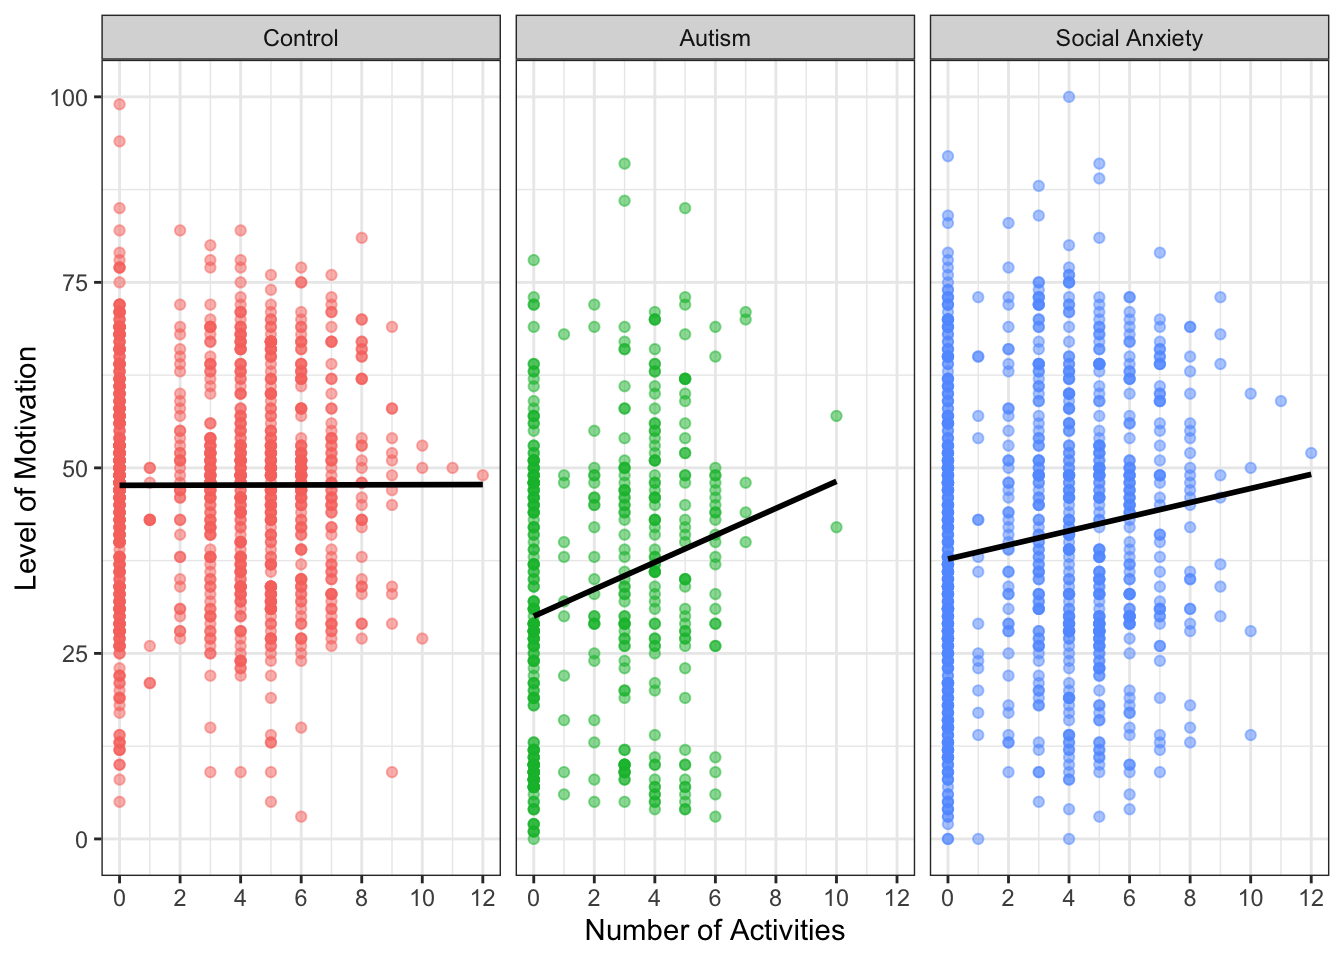
\includegraphics{04_results_files/figure-pdf/fig-Analy-1.pdf}

}

\caption{\label{fig-Analy}Motivation vs.~number of activities for all
three groups.}

\end{figure}%

This analysis revealed that, without accounting for FE, there is no
significant relationship between the number of activities and motivation
in the control group. However, for the autism group, a steep slope
indicates that as the number of activities increases, so does
motivation. The social anxiety group also shows a positive slope, though
less pronounced, suggesting a correlation between increased activities
and higher motivation levels. These findings contradict existing
literature, which support that motivation in the autism and social
anxiety groups should not necessarily rise with more activities,
underscoring the importance of using the FE model.

Figure~\ref{fig-FEAnaly} presents plots illustrating the influence of
activities on motivation. The dashed pooling line represents the
intercept and slope if all data were analyzed together, while the solid
lines show individual lines of best fit for each participant. This means
each individual has a different intercept, but all share the same slope.

\begin{figure}[H]

\centering{

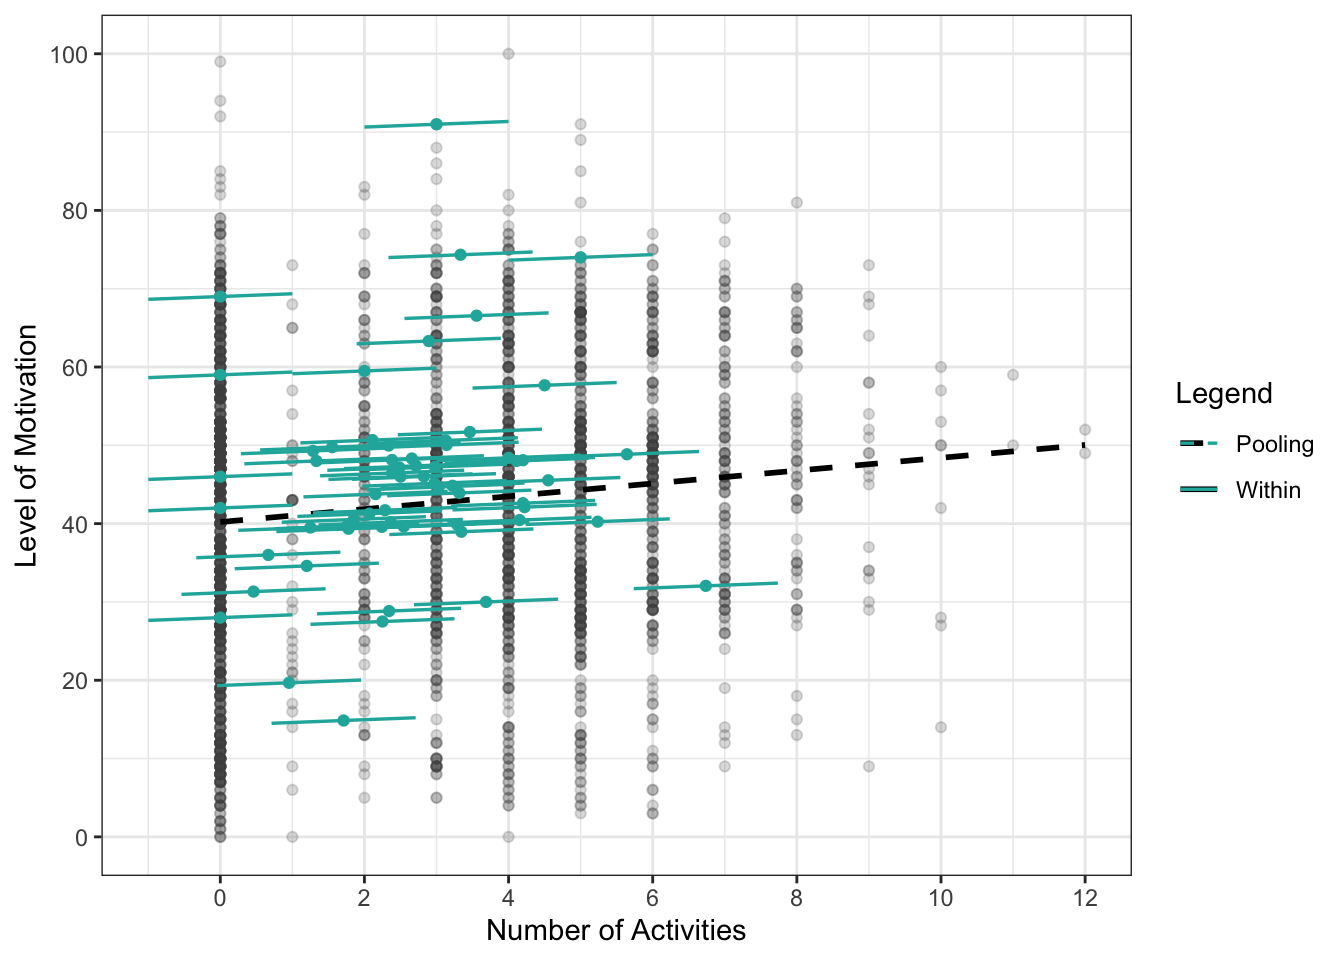
\includegraphics{04_results_files/figure-pdf/fig-FEAnaly-1.pdf}

}

\caption{\label{fig-FEAnaly}FE model for motivation vs.~number of
activities for all participants.}

\end{figure}%

While modeling each participant individually is crucial for accounting
for varying baseline levels of motivation, we found that applying a FE
model to each group---control, autism, and social anxiety---was also
important for understanding the true relationship between the number of
activities and motivation, as each group may have different baseline
levels.

Figure~\ref{fig-groupFE} presents the results of the FE models for all
three groups. These models predict motivation based on the number of
activities while considering both individual and group baseline
differences. This approach allows for a more accurate assessment of the
impact of activities on motivation within each distinct group. The plots
illustrate unique patterns for each group, emphasizing the value of
tailored analyses. Notably, the autism and social anxiety groups show
steeper slopes when all data are pooled together; however, when
individuals are analyzed separately, the slopes for each group are much
less steep. These results align more closely with expectations from
existing literature.

\begin{figure}[H]

\centering{

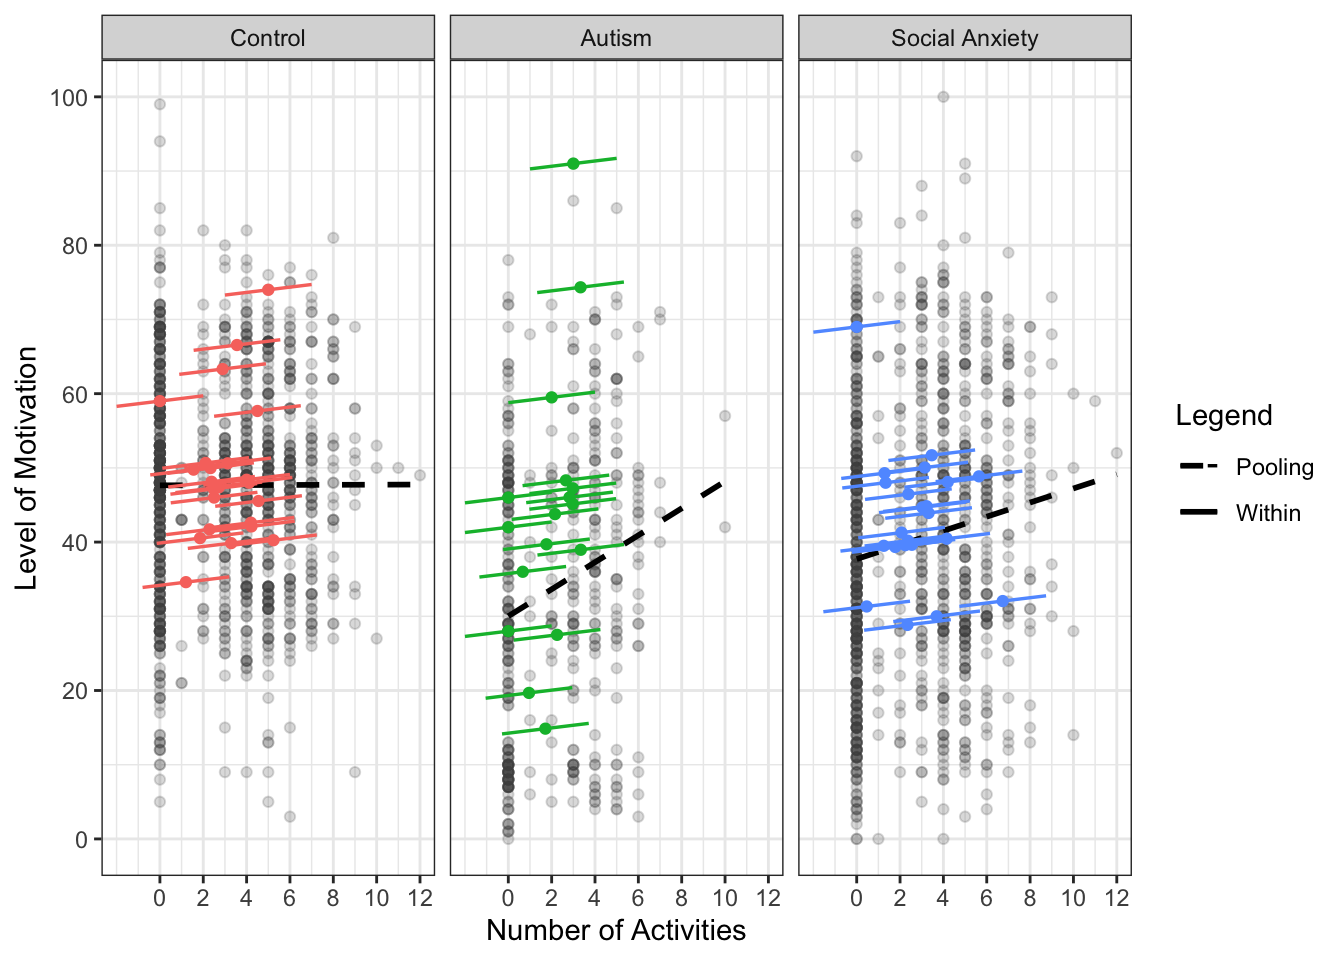
\includegraphics{04_results_files/figure-pdf/fig-groupFE-1.pdf}

}

\caption{\label{fig-groupFE}FE model for motivation vs.~number of
activities by group.}

\end{figure}%

Since the FE models require both an evening survey response for
motivation and the number of activities determined by the DBSCAN-TE
algorithm, some data were lost. This reduced the sample size from 31 to
23 in the control group, from 29 to 17 in the autism group, and from 28
to 22 in the social anxiety group. The FE models need enough data points
for each participant to ensure effective analysis, which explains the
reduction in participants. After visualizing the relationships, we
proceeded with running the FE models for each group. The results from
these models are presented in Table~\ref{tbl-groupFEAnaly}.

\begin{table}

\caption{\label{tbl-groupFEAnaly}FE Models: Motivation and Number of
Activities by Group}

\centering{

\centering
\begin{tabular}[t]{lccc}
\toprule
  & Group: Control & Group: Autism & Group: Social Anxiety\\
\midrule
No. of Activities & 0.259+ & 0.361 & 0.483*\\
 & (1.716) & (1.147) & (2.149)\\
\midrule
No. of Obs. & 1,167 & 451 & 1,033\\
AIC & 9,177.454 & 3,597.049 & 8,797.231\\
R² & 0.003 & 0.003 & 0.004\\
\bottomrule
\multicolumn{4}{l}{\rule{0pt}{1em}Robust t-statistics in parentheses. + p \$<\$ 0.1, * p \$<\$ 0.05, ** p \$<\$ 0.01, *** p \$<\$ 0.001}\\
\end{tabular}

}

\end{table}%

The FE models for the control, autism, and social anxiety groups
revealed different relationships between the number of activities and
motivation. For the control group, the coefficient was 0.259, suggesting
a marginally positive but not strongly significant relationship. In the
autism group, the coefficient was 0.361, also indicating a positive but
statistically insignificant relationship between activities and
motivation. However, the social anxiety group had a coefficient of
0.483, showing a statistically significant positive relationship. This
suggests that increasing activities is notably linked to higher
motivation for individuals with social anxiety.

These findings underscore the importance of recognizing individual
differences across groups. The significant positive relationship in the
social anxiety group suggests that increasing activities could be
particularly effective in enhancing motivation for this population. In
contrast, the control and autism groups did not show strong evidence of
this relationship, indicating that other factors might play a more
critical role in influencing motivation for these groups.

\subsubsection{Motivation and Suicidal
Ideation}\label{motivation-and-suicidal-ideation}

The prevalence of suicidal ideation across the groups underscores the
complex interplay between mental health and activity engagement. The
literature suggests that suicidal behavior is negatively associated with
overall well-being (Fonseca-Pedrero et al., 2022; Fumero et al., 2021).
Since we connected motivation to well-being, a similar association is
drawn between suicidal tendency and motivation.

Based on similar conclusions from the motivation and number of
activities analysis, we continued to perform the analysis by group.
Table~\ref{tbl-groupFESuic} shows the FE models for the impact of
suicidal intensity, which was scored from 1-100, on level of motivation,
which was also scored from 1-100, for individuals by group.

\begin{table}

\caption{\label{tbl-groupFESuic}FE Models: Motivation and Suicidal
Intensity by Group}

\centering{

\centering
\begin{tabular}[t]{lccc}
\toprule
  & Group: Autism & Group: Social Anxiety & Group: Control\\
\midrule
Suicidal Intesity & -0.095+ & -0.160*** & -0.361**\\
 & (-1.927) & (-5.518) & (-3.293)\\
\midrule
No. of Obs. & 484 & 822 & 66\\
AIC & 3,942.104 & 6,934.607 & 568.685\\
R² & 0.012 & 0.04 & 0.113\\
\bottomrule
\multicolumn{4}{l}{\rule{0pt}{1em}Robust t-statistics in parentheses. + p \$<\$ 0.1, * p \$<\$ 0.05, ** p \$<\$ 0.01, *** p \$<\$ 0.001}\\
\end{tabular}

}

\end{table}%

The FE models for the autism, social anxiety, and control groups show
distinct relationships between suicidal intensity and motivation levels.
In the autism group, the coefficient for suicidal intensity is -0.095,
indicating a marginally significant negative relationship, suggesting
that higher suicidal intensity may slightly reduce motivation, though
the evidence is weak. In contrast, the social anxiety group shows a
coefficient of -0.160, with a statistically significant negative
relationship, meaning higher suicidal intensity is strongly linked to
decreased motivation. Similarly, the control group's coefficient is
-0.361, with a significant negative relationship, showing that increased
suicidal intensity is associated with notably lower motivation levels.

These findings emphasize the need to consider the impact of suicidal
intensity on motivation within each group. While the relationship is
negative across all groups, the varying strength and significance
highlight the necessity for tailored interventions to address
motivational challenges in each population.

\subsection{Activity Types}\label{activity-types}

We examined how the number of activities at different locations---such
as parks, grocery stores, libraries, and social recreation
spaces---impacts motivation across each group. The analysis factored in
activity counts determined by the DBSCAN-TE algorithm, along with
seven-day and 14-day moving averages. While all activity locations and
measurements were included, only a few yielded statistically significant
results. Notably, significant findings emerged for the seven-day average
park activities and daily grocery store activities, highlighting their
potential influence on individual motivation levels.

\subsubsection{Activities at Parks}\label{activities-at-parks}

Table~\ref{tbl-groupFEParks} presents the FE models for the seven-day
rolling average number of activities at parks for the three groups.

\begin{table}

\caption{\label{tbl-groupFEParks}FE Models: Motivation and Number of
Activities at Parks by Group}

\centering{

\centering
\begin{tabular}[t]{lccc}
\toprule
  & Group: Control & Group: Autism & Group: Social Anxiety\\
\midrule
Seven-Day Park & 3.017* & 4.938 & 1.511\\
 & (2.239) & (0.857) & (0.207)\\
\midrule
No. of Obs. & 1,840 & 774 & 1,597\\
AIC & 14,509.34 & 6,215.856 & 13,615.11\\
R² & 0.002 & 0.001 & 0\\
\bottomrule
\multicolumn{4}{l}{\rule{0pt}{1em}Robust t-statistics in parentheses. + p \$<\$ 0.1, * p \$<\$ 0.05, ** p \$<\$ 0.01, *** p \$<\$ 0.001}\\
\end{tabular}

}

\end{table}%

In examining park activities, statistically significant results were
observed solely for the control group. A positive correlation emerged,
indicating that each additional park activity within a seven-day period
corresponded with a 3.017-point increase in motivation score. This
suggests that frequent park visits over a week are linked to heightened
motivation levels among individuals in the control group. Conversely,
the analysis did not unveil any significant correlation between park
visits and motivation levels for the autism and social anxiety groups.
This implies that park activities within the examined time frames do not
notably affect motivation levels for these groups.

\subsubsection{Activities at Grocery
Stores}\label{activities-at-grocery-stores}

Table~\ref{tbl-groupFEGrocery} presents the FE models for the number of
activities at grocery stores for the three groups.

\begin{table}

\caption{\label{tbl-groupFEGrocery}FE Models: Motivation and Number of
Activities at Grocery Stores by Group}

\centering{

\centering
\begin{tabular}[t]{lccc}
\toprule
  & Group: Control & Group: Autism & Group: Social Anxiety\\
\midrule
Grocery Store & -2.690+ & -2.725*** & 0.519\\
 & (-1.878) & (-3.721) & (0.614)\\
\midrule
No. of Obs. & 1,167 & 451 & 1,033\\
AIC & 9,178.666 & 3,598.227 & 8,801.453\\
R² & 0.002 & 0.001 & 0\\
\bottomrule
\multicolumn{4}{l}{\rule{0pt}{1em}Robust t-statistics in parentheses. + p \$<\$ 0.1, * p \$<\$ 0.05, ** p \$<\$ 0.01, *** p \$<\$ 0.001}\\
\end{tabular}

}

\end{table}%

The examination of grocery store visits unveiled intriguing trends
across the different groups. Notably, a statistically significant
negative correlation was found for the autism group, indicating a
decrease in motivation by 2.725 points with each additional grocery
store activity (p \textless{} 0.001). Similarly, the control group
exhibited a slight negative correlation (p \textless{} 0.1), with each
additional daily extra grocery store visit reducing motivation by 2.690
points. Conversely, no statistical significance was observed for the
social anxiety group. These findings underscore a nuanced connection
between grocery store visits and motivation, with notable negative
impacts identified in the autism group, while no significant
associations were evident in the control and social anxiety groups.

\subsubsection{Activity Impact on
Motivation}\label{activity-impact-on-motivation}

These findings are important because they reveal how activities impact
mental well-being differently for individuals with autism, social
anxiety, and those without these conditions. For the control group, the
positive correlation with seven-day average park visits suggests outdoor
activities benefit overall well-being. Conversely, the negative
correlation with grocery store visits for the autism group highlights
the stress linked to routine tasks like grocery shopping. Understanding
these differences is key to designing tailored interventions. For
example, promoting park visits could boost well-being in the general
population, while reducing stress in grocery environments could aid
autistic individuals. The lack of significant results for specific
locations in the social anxiety group suggests that overall activity
levels, rather than specific locations, may be more crucial to their
well-being.

\bookmarksetup{startatroot}

\section{Conclusions}\label{conclusions}

This study has provided valuable insights into the complex relationship
between travel behavior and mental health among young adults with
suicidal ideation. By analyzing LBS data and conducting statistical
modeling, we uncovered significant differences in activity engagement,
motivation levels, and suicidal ideation across different neurological
or physiological groups.

\subsection{Overall Implications}\label{overall-implications}

In this study, we explored the distinct differences in activity
engagement, motivation levels, and suicidal tendencies among individuals
in autism, social anxiety, and control groups to better understand the
unique challenges these populations face.

The study revealed that autistic individuals and individuals with social
anxiety engage in fewer activities compared to the control group,
indicating unique challenges in their daily routines and social
interactions. It also showed that motivation levels are lower in both
the autism and social anxiety groups compared to the control group,
highlighting the significant impact these conditions have on personal
drive. Specifically, the control group exhibited the highest motivation
levels, followed by the autism group, with the social anxiety group
having the lowest. Additionally, a correlation was found between
increased suicidal intensity and decreased motivation across all groups,
with the social anxiety group reporting the highest frequency of
suicidal thoughts.

We also identified a minimal positive relationship between the number of
activities and motivation, suggesting that simply increasing activity
engagement is not enough to significantly enhance motivation. Moreover,
a negative relationship between travel distance and motivation was
observed, indicating that longer travel distances slightly decrease
motivation, though the effect is relatively minor. Ultimately, adjusting
either of these aspects of travel would not be a sufficient strategy for
significantly boosting motivation for individuals.

Overall, these findings highlight significant differences in activity
engagement, motivation levels, and suicidality among individuals with
autism, social anxiety, and the control group. They underscore the need
for tailored approaches to address the unique challenges faced by each
group.

\subsection{Group Specific
Implications}\label{group-specific-implications}

Different types of activities had varying effects on motivation levels
across the groups studied. For individuals with social anxiety, a
positive relationship was observed between the number of activities
engaged in and their motivation levels, indicating that increased
activity participation could enhance their well-being. Conversely, for
autistic individuals, there was a negative correlation between grocery
store visits and motivation levels, suggesting that grocery store
environments may present stressors that adversely affect their
well-being. These findings are important as they provide insight into
the distinct challenges faced by individuals with social anxiety and
autism. Additionally, the strong positive correlation between seven-day
average park visits and motivation levels in the control group
highlights the beneficial impact of outdoor green-space activities on
well-being.

In summary, each group benefits differently from various activities,
underscoring the importance of personalized approaches to improving
well-being tailored to the specific needs and preferences of individuals
in each group.

\subsection{Significance}\label{significance}

In this research, we explored the critical link between travel behavior
and mental health, focusing on young adults with suicidal ideation. By
analyzing daily activities and movement patterns, the study highlights
the importance of considering these factors in mental health
interventions. The contributions of this work bridge the gap between
travel behavior and mental health research, emphasizing the need for
personalized approaches that take into account the unique challenges
faced by individuals with autism and social anxiety.

The study reveals that individuals with autism and social anxiety engage
in fewer activities and have lower motivation levels compared to the
control group, underscoring the significant impact of these conditions
on daily life. Additionally, the correlation between suicidal ideation
and decreased motivation across all groups highlights critical areas for
intervention and prevention.

The practical implications of these findings are significant. By
understanding how travel behavior influences motivation levels and
well-being, mental health practitioners can develop targeted strategies
to support individuals struggling with mental health challenges. For
example, interventions can be tailored to address specific needs related
to travel patterns, such as mitigating stressors in grocery store
environments for autistic individuals or encouraging activity engagement
for those with social anxiety.

Overall, this research underscores the importance of considering travel
behavior as a key factor in promoting mental well-being. It offers a
roadmap for future studies to explore this intersection further,
ultimately aiming to enhance the quality of life for individuals by
informing more personalized and effective mental health strategies.

\bookmarksetup{startatroot}

\section{Limitations and Future
Recommendations}\label{limitations-and-future-recommendations}

There are some important limitations and future considerations following
the analysis of the BYU CAPS data. These limitations are due to
potential issues with data collection, lack of activities duration from
the DBSCAN-TE algorithm, and the inability to confirm activity
engagement for the participants.

\subsection{Data Collection}\label{data-collection}

The primary limitation of this study pertains to the quality of the data
of the participants. Since participants participated for varying lengths
of time and their phones were not always on to collect LBS data, the
data was sometimes sparse. Even though a substantial amount of data had
to be discarded due to poor quality, influenced by factors such as
participants turning off their phones or the app failing to record data
accurately, we did our best to accurately account for the well-being and
activity patterns of the individuals. The inconsistency in data
collection may have made it difficult for the DBSCAN-TE algorithm to
perfectly identify activities. While it performed with 91.5\% accuracy,
some of the activity days that were manually checked appeared to be
missing identified activities. Additionally, since the userID-activity
days needed corresponding mental health data and activity data, we tried
to account for the gaps by imputing the number of activities for a
seven-day rolling average number of activities and by calculating the
convex hull area and the distance traveled.

To address these limitations in future studies, improving data quality
would be paramount. Strategies could include implementing measures to
encourage consistent phone usage among participants or enhancing the
app's reliability in recording data accurately. Additionally,
incorporating redundancy measures within the data collection process,
such as cross-referencing data from multiple sources or employing
complementary data collection methods, could help mitigate the impact of
sporadic data collection. Moreover, refining the DBSCAN-TE algorithm to
improve accuracy in identifying activities, potentially through machine
learning techniques or incorporating additional contextual information,
could enhance the reliability of activity data. By prioritizing efforts
to enhance data quality and implementing more robust data collection and
processing procedures, future studies can better capture and analyze
individuals' mental health and activity patterns, thereby yielding
additional findings.

\subsection{Activity Duration}\label{activity-duration}

The study also lacks detailed information on the duration of
participants' activities. While the dataset indicates that certain
activities occurred, it does not specify how long participants spent
engaging in these activities. For example, we know whether participants
visited parks, but not the duration of their stay at the park. This
limitation means we cannot accurately assess the impact of time spent in
specific environments on mental well-being. Additionally, since the
algorithm determined activities based on relatively stationary LBS data,
we did not account for instances where participants might have merely
passed through green-spaces or parks without spending significant time
there. This omission further complicates our understanding of the
relationship between activities and mental health. These limitations
highlight the challenges in using mobile-based data collection for
mental health research.

Future studies could focus on improving the accuracy of
location-tracking algorithms, ensuring consistent data collection, and
capturing detailed activity duration to provide a more comprehensive
understanding of the interaction between travel behavior and mental
well-being.

\subsection{Activity Diaries}\label{activity-diaries}

One other potential limitation of our study is the inability to confirm
which specific activities individuals participated in throughout the
day. While we have identified activities using the DBSCAN-TE algorithm,
there is a possibility that certain activities were not accurately
identified by the algorithm, leading to their omission from our
analysis. This lack of precision could potentially result in some
activities going undetected, thereby limiting the comprehensiveness of
our activity analysis.

To address this limitation in future research, integrating activity
diaries into survey methodology could prove beneficial. By incorporating
activity diaries, participants would have the opportunity to provide
detailed accounts of their daily activities, including specific
locations where these activities took place. This additional information
could enhance the completeness and accuracy of our activity analysis, as
it would provide valuable insights into the types and locations of
activities individuals engage in throughout the day.

\subsection{Overall Recommendations}\label{overall-recommendations}

To build on the findings of this study and address its limitations,
future research should prioritize the following:

\begin{itemize}
\item
  Enhance Data Collection Methods: Consider using multiple data sources
  or complementary methods to ensure comprehensive data capture. Invest
  in refining activity identification algorithms and explore advanced
  machine learning techniques to improve accuracy and reduce gaps in
  activity data.
\item
  Capture Detailed Activity Duration: Focus on capturing both activity
  types and durations by implementing time-tracking features to better
  understand the impact of activities on mental well-being.
\item
  Implement Participant Activity Diaries: Integrate activity diaries to
  confirm activity engagement and duration. Enhance the completeness and
  accuracy of daily activity engagement.
\end{itemize}

By addressing these recommendations, future studies can improve the
quality of data, enhance the accuracy of activity analysis, and provide
a more comprehensive understanding of the interplay between activity
patterns and mental health.

\bookmarksetup{startatroot}

\section*{Acknowledgments}\label{acknowledgments}
\addcontentsline{toc}{section}{Acknowledgments}

\markboth{Acknowledgments}{Acknowledgments}

This data used in this research was collected with help from an
Interdisciplinary Research Grant at Brigham Young University, and
administered under IRB protocol F2020-242. The investigators on the
overarching grant include Terisa Gabrielsen, Jared Nielsen, and Mikle
South.

\bookmarksetup{startatroot}

\section*{References}\label{references}
\addcontentsline{toc}{section}{References}

\markboth{References}{References}

\phantomsection\label{refs}
\begin{CSLReferences}{1}{0}
\bibitem[\citeproctext]{ref-aylottExploratoryStudyGrocery1998}
Aylott, R., \& Mitchell, V.-W. (1998). An exploratory study of grocery
shopping stressors. \emph{International Journal of Retail \&
Distribution Management}, \emph{26}(9), 362--373.
\url{https://doi.org/10.1108/09590559810237908}

\bibitem[\citeproctext]{ref-baileyRelationshipSocialExperience2020}
Bailey, K. M., Frost, K. M., Casagrande, K., \& Ingersoll, B. (2020).
The relationship between social experience and subjective well-being in
autistic college students: {A} mixed methods study. \emph{Autism},
\emph{24}(5), 1081--1092. \url{https://doi.org/10.1177/1362361319892457}

\bibitem[\citeproctext]{ref-barryAddressingDeterminantsPositive2009}
Barry, M. M. (2009). Addressing the determinants of positive mental
health: {Concepts}, evidence and practice. \emph{International Journal
of Mental Health Promotion}, \emph{11}(3), 4--17.
\url{https://doi.org/10.1080/14623730.2009.9721788}

\bibitem[\citeproctext]{ref-brewsterPublicLibraryTherapeutic2014}
Brewster, L. (2014). The public library as therapeutic landscape: {A}
qualitative case study. \emph{Health \& Place}, \emph{26}, 94--99.
\url{https://doi.org/10.1016/j.healthplace.2013.12.015}

\bibitem[\citeproctext]{ref-dekaTravelPatternsNeeds2016}
Deka, D., Feeley, C., \& Lubin, A. (2016). Travel patterns, needs, and
barriers of adults with autism spectrum disorder: {Report} from a
survey. \emph{Transportation Research Record}, \emph{2542}(1), 9--16.
\url{https://doi.org/10.3141/2542-02}

\bibitem[\citeproctext]{ref-delboscExploringRelativeInfluences2011}
Delbosc, A., \& Currie, G. (2011). Exploring the relative influences of
transport disadvantage and social exclusion on well-being.
\emph{Transport Policy}, \emph{18}(4), 555--562.
\url{https://doi.org/10.1016/j.tranpol.2011.01.011}

\bibitem[\citeproctext]{ref-eliaPublicLibrariesSupporting2019}
Elia, H. (2019). Public libraries supporting health and wellness: {A}
literature review. \emph{School of Information Student Research
Journal}, \emph{9}(2). \url{https://doi.org/10.31979/2575-2499.090207}

\bibitem[\citeproctext]{ref-fonseca-pedreroRiskProtectiveFactors2022}
Fonseca-Pedrero, E., Al-Halabí, S., Pérez-Albéniz, A., \& Debbané, M.
(2022). Risk and protective factors in adolescent suicidal behaviour:
{A} network analysis. \emph{International Journal of Environmental
Research and Public Health}, \emph{19}(3), 1784.
\url{https://doi.org/10.3390/ijerph19031784}

\bibitem[\citeproctext]{ref-frimanHowDoesTravel2017}
Friman, M., Gärling, T., Ettema, D., \& Olsson, L. E. (2017). How does
travel affect emotional well-being and life satisfaction?
\emph{Transportation Research Part A: Policy and Practice}, \emph{106},
170--180. \url{https://doi.org/10.1016/j.tra.2017.09.024}

\bibitem[\citeproctext]{ref-fumeroAdolescentsBipolarExperiences2021}
Fumero, A., Marrero, R. J., Pérez-Albéniz, A., \& Fonseca-Pedrero, E.
(2021). Adolescents' bipolar experiences and suicide risk: {Well-being}
and mental health difficulties as mediators. \emph{International Journal
of Environmental Research and Public Health}, \emph{18}(6), 3024.
\url{https://doi.org/10.3390/ijerph18063024}

\bibitem[\citeproctext]{ref-hoisingtonTenQuestionsConcerning2019}
Hoisington, A. J., Stearns-Yoder, K. A., Schuldt, S. J., Beemer, C. J.,
Maestre, J. P., Kinney, K. A., Postolache, T. T., Lowry, C. A., \&
Brenner, L. A. (2019). Ten questions concerning the built environment
and mental health. \emph{Building and Environment}, \emph{155}, 58--69.
\url{https://doi.org/10.1016/j.buildenv.2019.03.036}

\bibitem[\citeproctext]{ref-kennyWhichTermsShould2016}
Kenny, L., Hattersley, C., Molins, B., Buckley, C., Povey, C., \&
Pellicano, E. (2016). Which terms should be used to describe autism?
{Perspectives} from the {UK} autism community. \emph{Autism},
\emph{20}(4), 442--462. \url{https://doi.org/10.1177/1362361315588200}

\bibitem[\citeproctext]{ref-kuykendallLeisureEngagementSubjective2015}
Kuykendall, L., Tay, L., \& Ng, V. (2015). Leisure engagement and
subjective well-being: {A} meta-analysis. \emph{Psychological Bulletin},
\emph{141}(2), 364--403. \url{https://doi.org/10.1037/a0038508}

\bibitem[\citeproctext]{ref-lanDailySpacetimeActivities2022}
Lan, Y., Roberts, H., Kwan, M.-P., \& Helbich, M. (2022). Daily
space-time activities, multiple environmental exposures, and anxiety
symptoms: {A} cross-sectional mobile phone-based sensing study.
\emph{Science of The Total Environment}, \emph{834}, 155276.
\url{https://doi.org/10.1016/j.scitotenv.2022.155276}

\bibitem[\citeproctext]{ref-leichsenringSocialAnxietyDisorder2017}
Leichsenring, F., \& Leweke, F. (2017). Social anxiety disorder.
\emph{New England Journal of Medicine}, \emph{376}(23), 2255--2264.
\url{https://doi.org/10.1056/NEJMcp1614701}

\bibitem[\citeproctext]{ref-loadesRapidSystematicReview2020}
Loades, M. E., Chatburn, E., Higson-Sweeney, N., Reynolds, S., Shafran,
R., Brigden, A., Linney, C., McManus, M. N., Borwick, C., \& Crawley, E.
(2020). Rapid systematic review: {The} impact of social isolation and
loneliness on the mental health of children and adolescents in the
context of {COVID-19}. \emph{Journal of the American Academy of Child \&
Adolescent Psychiatry}, \emph{59}(11), 1218--1239.e3.
\url{https://doi.org/10.1016/j.jaac.2020.05.009}

\bibitem[\citeproctext]{ref-lubinTransportationIssuesAdults2016}
Lubin, A., \& Feeley, C. (2016). Transportation issues of adults on the
autism spectrum: {Findings} from focus group discussions.
\emph{Transportation Research Record}, \emph{2542}(1), 1--8.
\url{https://doi.org/10.3141/2542-01}

\bibitem[\citeproctext]{ref-macfarlaneClassifyingLocationPoints2024}
Macfarlane, G. S., Riches, G., Youngs, E. K., \& Nielsen, J. A. (2024).
Classifying location points as daily activities using simultaneously
optimized {DBSCAN-TE} parameters. \emph{Findings}.
\url{https://doi.org/10.32866/001c.116197}

\bibitem[\citeproctext]{ref-mackettMentalHealthTravel2021}
Mackett, R. L. (2021). Mental health and travel behaviour. \emph{Journal
of Transport \& Health}, \emph{22}, 101143.
\url{https://doi.org/10.1016/j.jth.2021.101143}

\bibitem[\citeproctext]{ref-MentalHealthNumbers2023}
Mental {Health By} the {Numbers}. (2023). In \emph{NAMI}.

\bibitem[\citeproctext]{ref-nilssonEffectsTimePressure2017}
Nilsson, E., Gärling, T., \& Marell, A. (2017). Effects of time
pressure, type of shopping, and store attributes on consumers'
satisfaction with grocery shopping. \emph{The International Review of
Retail, Distribution and Consumer Research}, \emph{27}(4), 334--351.
\url{https://doi.org/10.1080/09593969.2017.1309674}

\bibitem[\citeproctext]{ref-orbenEffectsSocialDeprivation2020}
Orben, A., Tomova, L., \& Blakemore, S.-J. (2020). The effects of social
deprivation on adolescent development and mental health. \emph{The
Lancet Child \& Adolescent Health}, \emph{4}(8), 634--640.
\url{https://doi.org/10.1016/S2352-4642(20)30186-3}

\bibitem[\citeproctext]{ref-ozturkRelationshipAttachmentStyle2010}
Öztürk, A., \& Mutlu, T. (2010). The relationship between attachment
style, subjective well-being, happiness and social anxiety among
university students'. \emph{Procedia - Social and Behavioral Sciences},
\emph{9}, 1772--1776. \url{https://doi.org/10.1016/j.sbspro.2010.12.398}

\bibitem[\citeproctext]{ref-pelgrimsAssociationUrbanEnvironment2021}
Pelgrims, I., Devleesschauwer, B., Guyot, M., Keune, H., Nawrot, T. S.,
Remmen, R., Saenen, N. D., Trabelsi, S., Thomas, I., Aerts, R., \& De
Clercq, E. M. (2021). Association between urban environment and mental
health in {Brussels}, {Belgium}. \emph{BMC Public Health}, \emph{21}(1),
635. \url{https://doi.org/10.1186/s12889-021-10557-7}

\bibitem[\citeproctext]{ref-pousoContactBluegreenSpaces2021}
Pouso, S., Borja, Á., Fleming, L. E., Gómez-Baggethun, E., White, M. P.,
\& Uyarra, M. C. (2021). Contact with blue-green spaces during the
{COVID-19} pandemic lockdown beneficial for mental health. \emph{Science
of The Total Environment}, \emph{756}, 143984.
\url{https://doi.org/10.1016/j.scitotenv.2020.143984}

\bibitem[\citeproctext]{ref-rateringMovingAnxietyDisorder2024}
Ratering, C., van der Heijden, R., \& Martens, K. (2024). Moving around
with an anxiety disorder. \emph{Transportation Research Part F: Traffic
Psychology and Behaviour}, \emph{100}, 493--506.
\url{https://doi.org/10.1016/j.trf.2023.12.005}

\bibitem[\citeproctext]{ref-rautioLivingEnvironmentIts2018}
Rautio, N., Filatova, S., Lehtiniemi, H., \& Miettunen, J. (2018).
Living environment and its relationship to depressive mood: {A}
systematic review. \emph{International Journal of Social Psychiatry},
\emph{64}(1), 92--103. \url{https://doi.org/10.1177/0020764017744582}

\bibitem[\citeproctext]{ref-richesTransformingGPSPoints2022}
Riches, G. (2022). \emph{Transforming {GPS} points to daily activities
using simultaneously optimized {DBSCAN-TE} parameters}. MS Thesis,
Brigham Young University.

\bibitem[\citeproctext]{ref-ridgwaySubjectiveWellbeingAutistic}
Ridgway, K., Macmillan, C., Demmer, D. H., Hooley, M., Hedley, D.,
Westrupp, E., \& Stokes, M. A. (2024). Subjective wellbeing of autistic
adolescents and young adults: {A} cross sectional study. \emph{Autism
Research}, \emph{n/a}(n/a). \url{https://doi.org/10.1002/aur.3139}

\bibitem[\citeproctext]{ref-stanleyMobilitySocialExclusion2011}
Stanley, J. K., Hensher, D. A., Stanley, J. R., \& Vella-Brodrick, D.
(2011). Mobility, social exclusion and well-being: {Exploring} the
links. \emph{Transportation Research Part A: Policy and Practice},
\emph{45}(8), 789--801. \url{https://doi.org/10.1016/j.tra.2011.06.007}

\bibitem[\citeproctext]{ref-syahputriEffectTravelSatisfaction2022}
Syahputri, J., Dharmowijoyo, D. B. E., Basuki Joewono, T., \& Rizki, M.
(2022). Effect of travel satisfaction and heterogeneity of
activity-travel patterns of other persons in the household on social and
mental health: {The} case of {Bandung Metropolitan} area. \emph{Case
Studies on Transport Policy}, \emph{10}(4), 2111--2124.
\url{https://doi.org/10.1016/j.cstp.2022.09.005}

\bibitem[\citeproctext]{ref-takiguchiRelationshipLeisureActivities2022}
Takiguchi, Y., Matsui, M., Kikutani, M., \& Ebina, K. (2022). The
relationship between leisure activities and mental health: {The} impact
of resilience and {COVID}-19. \emph{Applied Psychology. Health and
Well-Being}, 10.1111/aphw.12394.
\url{https://doi.org/10.1111/aphw.12394}

\bibitem[\citeproctext]{ref-whiteAssociationsGreenBlue2021}
White, M. P., Elliott, L. R., Grellier, J., Economou, T., Bell, S.,
Bratman, G. N., Cirach, M., Gascon, M., Lima, M. L., Lõhmus, M.,
Nieuwenhuijsen, M., Ojala, A., Roiko, A., Schultz, P. W., van den Bosch,
M., \& Fleming, L. E. (2021). Associations between green/blue spaces and
mental health across 18 countries. \emph{Scientific Reports},
\emph{11}(1), 8903. \url{https://doi.org/10.1038/s41598-021-87675-0}

\bibitem[\citeproctext]{ref-wooldridgeIntroductoryEconometricsModern2009}
Wooldridge, J. (2009). \emph{Introductory {Econometrics}: {A Modern
Appraoch}} (4th ed.). South-Western Cengage Learning. Mason, Ohio.

\bibitem[\citeproctext]{ref-yanosNegativeSupportiveSocial2001}
Yanos, P. T., Rosenfield, S., \& Horwitz, A. V. (2001). Negative and
supportive social interactions and quality of life among persons
diagnosed with severe mental illness. \emph{Community Mental Health
Journal}, \emph{37}(5), 405--419.
\url{https://doi.org/10.1023/A:1017528029127}

\bibitem[\citeproctext]{ref-yeSocialAnxietySubjective2021}
Ye, B., Li, L., Wang, P., Wang, R., Liu, M., Wang, X., \& Yang, Q.
(2021). Social anxiety and subjective well-being among {Chinese} college
students: {A} moderated mediation model. \emph{Personality and
Individual Differences}, \emph{175}, 110680.
\url{https://doi.org/10.1016/j.paid.2021.110680}

\end{CSLReferences}



\end{document}
